\section*{\lr{2.6} جدول معنایی}

      روش جدول معنایی یک رویهٔ تصمیم‌گیری کارآمد برای بررسی ارضاپذیری (و به‌طور دوگانه، همگانی‌صدقی) در منطق گزاره‌ای است.  
      در فصل بعد، از جدول معنایی به‌طور گسترده برای اثبات قضایای مهم در مورد سیستم‌های استنتاجی استفاده خواهیم کرد.
      
      اصل بنیادین جدول معنایی بسیار ساده است:  
      با تجزیهٔ فرمول به مجموعه‌هایی از اتم‌ها و نقیض آن‌ها، در پی یافتن مدلی (تعبیری ارضاکننده) برای فرمول هستیم.
      
      بررسی امکان ارضا برای هر یک از این مجموعه‌ها آسان است:  
      یک مجموعه از اتم‌ها و نقیض اتم‌ها ارضاپذیر است اگر و تنها اگر شامل اتمی و نقیض همان اتم نباشد.  
      در نتیجه، فرمول اولیه ارضاپذیر است اگر حداقل یکی از این مجموعه‌ها ارضاپذیر باشد.
      
      اکنون با چند تعریف آغاز می‌کنیم و سپس ارضاپذیری دو فرمول را تحلیل می‌کنیم تا انگیزه‌ای برای ساختار جدول معنایی فراهم شود.

\subsection*{\lr{2.6.1} تجزیهٔ فرمول‌ها به مجموعه‌ای از لفظ‌ها}
  \begin{definition}[تعریف \lr{2.57}]
    یک \emph{لفظ} (literal)، یا \emph{اتم} است یا \emph{نفی یک اتم}.
    \begin{itemize}
      \item یک اتم، \emph{لفظِ مثبت} نامیده می‌شود.
      \item نفی یک اتم، \emph{لفظِ منفی} نام دارد.
    \end{itemize}
    برای هر اتم $p$، مجموعهٔ $\{p,\;\neg p\}$ یک \emph{زوج متمم} از لفظ‌ها تشکیل می‌دهد.  
    برای هر فرمول $A$، مجموعهٔ $\{A,\;\neg A\}$ نیز یک \emph{زوج متمم از فرمول‌ها} است.  
    فرمول $A$ متمم $\neg A$ و بالعکس است.
  \end{definition}
    
  \begin{example}[مثال \lr{2.58}]
    در مجموعهٔ لفظ‌ها
    \[
    \{\neg p,\; q,\; r,\; \neg r\}
    \]
    \begin{itemize}
      \item $q$ و $r$ لفظِ \emph{مثبت} هستند،
      \item $\neg p$ و $\neg r$ لفظِ \emph{منفی} هستند.
    \end{itemize}
    این مجموعه شامل زوج متمم $\{r,\neg r\}$ است.
  \end{example}
    
  \begin{example}[مثال \lr{2.59}]
    فرمول زیر را تحلیل می‌کنیم تا ارضاپذیری آن را در تعبیر دلخواه $\mathscr{I}$ بررسی کنیم:
    \[
    A = p \land (\neg q \lor \neg p).
    \]
    با استفاده از قواعد بازگشتی ارزیابی صدق:
    \begin{align*}
    v_{\mathscr{I}}(A)=T
    &\;\Longleftrightarrow\;
    v_{\mathscr{I}}(p)=T
    \;\land\;
    v_{\mathscr{I}}(\neg q\lor\neg p)=T,\\
    v_{\mathscr{I}}(\neg q\lor\neg p)=T
    &\;\Longleftrightarrow\;
    v_{\mathscr{I}}(\neg q)=T
    \;\lor\;
    v_{\mathscr{I}}(\neg p)=T.
    \end{align*}
    در نتیجه، $v_{\mathscr{I}}(A)=T$ اگر و تنها اگر یکی از دو حالت زیر برقرار باشد:
    \begin{enumerate}
      \item $v_{\mathscr{I}}(p)=T$ و $v_{\mathscr{I}}(\neg q)=T$
      \item $v_{\mathscr{I}}(p)=T$ و $v_{\mathscr{I}}(\neg p)=T$
    \end{enumerate}
    پس مسئلهٔ ارضاپذیری $A$ به بررسی ارضاپذیری دو مجموعهٔ لفظ‌ها کاهش می‌یابد.
  \end{example}
    
  \begin{theorem}[قضیه \lr{2.60}]
    مجموعه‌ای از لفظ‌ها \emph{ارضاپذیر} است \emph{اگر و تنها اگر} شامل هیچ \emph{زوج متممی} از لفظ‌ها نباشد.
  \end{theorem}
    
  \begin{proof}
    فرض کنید $L$ مجموعه‌ای از لفظ‌ها باشد که هیچ زوج متممی در آن وجود ندارد. تعبیر $\mathscr{I}$ را به‌صورت زیر تعریف می‌کنیم:
    \[
    \mathscr{I}(p)=
    \begin{cases}
    T, & \text{اگر  } p\in L,\\
    F, & \text{اگر  } \neg p\in L.
    \end{cases}
    \]
    این تعریف \emph{سازگار و کامل} است، زیرا در $L$ هیچ اتمی همراه نقیضش حضور ندارد. هر لفظِ موجود در $L$ در این تعبیر مقدار $T$ می‌گیرد؛ بنابراین $L$ ارضاپذیر است.
    
    حال اگر $\{p,\neg p\}\subseteq L$، در هر تعبیر ممکن یا $v_{\mathscr{I}}(p)=F$ یا $v_{\mathscr{I}}(\neg p)=F$ است، پس $L$ ارضاپذیر نخواهد بود.
  \end{proof}
    
  \begin{example}[مثال \lr{2.61}]
    ادامهٔ مثال \lr{2.59}:  
    برای $A = p\land(\neg q\lor\neg p)$، دو مجموعه‌ای که باید بررسی شوند:
    \[
    \{p,\neg p\}\quad\longrightarrow\quad\text{دارای زوج متمم}\;\to\;\text{ناتوان از ارضا},
    \]
    \[
    \{p,\neg q\}\quad\longrightarrow\quad\text{فاقد زوج متمم}\;\to\;\text{ارضاپذیر}.
    \]
    بنابراین فقط مجموعهٔ دوم ارضاپذیر است و از قضیهٔ \lr{2.60} تعبیری به‌دست می‌آید که در آن
    \[
    \mathscr{I}(p)=T,\quad \mathscr{I}(q)=F.
    \]
  \end{example}
    
  \begin{example}[مثال \lr{2.62}]
    اگر فرمول \emph{ناتوان از ارضا} باشد، مثلاً:
    \[
    B = (p\lor q)\land(\neg p\land\neg q),
    \]
    آنگاه:
    \begin{enumerate}
      \item برای ارضا شدن $B$ باید
        $v_{\mathscr{I}}(p\lor q)=T$ و $v_{\mathscr{I}}(\neg p\land\neg q)=T$.
      \item تجزیهٔ ترکیب عطفی و ترکیب فصلی نشان می‌دهد که دو حالت ممکن به مجموعه‌های لفظ‌ها می‌انجامد:
        \[
        \{p,\neg p,\neg q\},\quad \{q,\neg p,\neg q\}.
        \]
      \item هر دو شامل زوج متمم‌اند؛ بنابراین ناتوان از ارضا هستند (قضیهٔ \lr{2.60}).
    \end{enumerate}
    نتیجه می‌گیریم که \emph{هیچ مدلی برای $B$ وجود ندارد}، یعنی
    \[
   \text{ناتوان از ارضا است.} B\
    \]
  \end{example}
  
  \begin{figure}[ht]
    \centering
    \begin{latin}
      \resizebox{0.35\textwidth}{!}{
      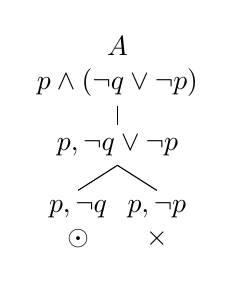
\begin{tikzpicture}[
        level distance=1cm,
        sibling distance=1.5cm,
        level 2/.style={sibling distance=1cm},
        edge from parent path={(\tikzparentnode.south) -- (\tikzchildnode.north)}
      ]
      \node[align=center] {$A$ \\ $p \land (\neg q \lor \neg p)$}
        child { 
          node {$p, \neg q \lor \neg p$}
          child { node[align=center] {$p, \neg q$ \\ $\odot$} }
          child { node[align=center] {$p, \neg p$ \\ $\times$} }
        };
      \end{tikzpicture}
      }
    \hfill
    \resizebox{0.35\textwidth}{!}{
      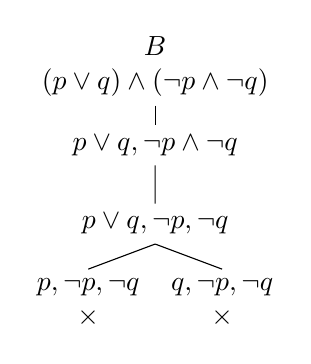
\begin{tikzpicture}[
        level distance=1cm,
        sibling distance=1.5cm,
        level 2/.style={sibling distance=1cm},
        level 3/.style={sibling distance=1.7cm},
        edge from parent path={(\tikzparentnode.south) -- (\tikzchildnode.north)}
      ]
      \node[align=center] {$B$ \\ $(p \lor q) \land (\neg p \land \neg q)$}
        child { 
          node {$p \lor q, \neg p \land \neg q$}
          child {
            node {$p \lor q, \neg p, \neg q$}
            child { node[align=center] {$p, \neg p, \neg q$ \\ $\times$} }
            child { node[align=center] {$q, \neg p, \neg q$ \\ $\times$} }
          }
        };
      \end{tikzpicture}
      }
    \end{latin}
    \renewcommand{\thefigure}{\lr{2.7}}
    \caption{درخت صدق}
  \end{figure}
\subsection*{\lr{2.6.2} ساخت جدول معنایی \lr{(Construction of Semantic Tableaux)}}
  
  تجزیهٔ فرمول به مجموعه‌ای از \emph{لفظ‌ها} در قالب متنی دشوار است. در روش \emph{جدول معنایی}، مجموعه‌های فرمول برچسبِ گره‌های یک درخت را تشکیل می‌دهند، به‌طوری که هر مسیر در درخت نمایانگر فرمول‌هایی است که باید در یک تعبیر ممکن صدق‌پذیر شوند.
  
  \begin{itemize}
    \item فرمول اولیه برچسبِ ریشهٔ درخت است.
    \item هر گره، بسته به نوع فرمول برچسب‌خورده، یک یا دو فرزند دارد.
    \item برگ‌ها با مجموعه‌ای از \emph{لفظ‌ها} برچسب می‌خورند.
    \item برگ‌هایی که شامل یک \emph{زوج متمم از لفظ‌ها} باشند با «$\times$» (بسته) و برگ‌هایی که فاقد زوج متمم هستند با $\odot$ (باز) علامت‌گذاری می‌شوند.
  \end{itemize}
  
  شکل \lr{2.7} جدول‌های معنایی مثال‌های پیشین را نشان می‌دهد. جدول زیر نمونهٔ دیگری از جدول معنایی برای فرمول
  \[
  B = (p \lor q)\;\land\;(\neg p \land \neg q)
  \]
  را نمایش می‌دهد که ابتدا برای $p \lor q$ منشعب شده و سپس $\neg p \land \neg q$ را پردازش می‌کند. واضح است که اگر \emph{همگرایی} ($\land$) را پیش از \emph{جمع‌گزاره} ($\lor$) بگشاییم، تعداد گره‌ها کمتر خواهد بود و در نتیجه کارآمدتر است.
  
  \begin{figure}[ht]
    \centering
    \begin{latin}
      \resizebox{0.35\textwidth}{!}{
      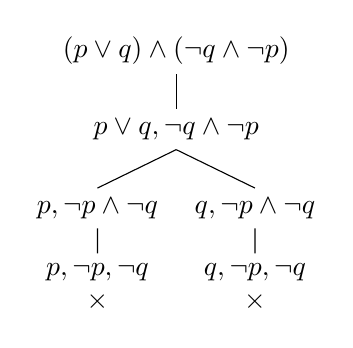
\begin{tikzpicture}[
        level distance=1cm,
        sibling distance=1.5cm,
        level 2/.style={sibling distance=2cm},
        level 2/.style={sibling distance=2cm},
        edge from parent path={(\tikzparentnode.south) -- (\tikzchildnode.north)}
      ]
      \node {$(p \lor q) \land (\neg q \land \neg p)$}
        child { 
          node {$p \lor q, \neg q \land \neg p$}
          child { 
            node {$p, \neg p \land \neg q$}
            child { node[align=center] {$p, \neg p, \neg q$ \\ $\times$} }
          }
          child { 
            node {$q, \neg p \land \neg q$}
            child { node[align=center] {$q, \neg p, \neg q$ \\ $\times$} }
          }
        };
      \end{tikzpicture}
      }
    \end{latin}
  \end{figure}
  
  برای ساده‌سازی و ایجاز، فرمول‌ها را بر اساس \emph{اپراتور اصلی} شان به دو دستهٔ \emph{$\alpha$-فرمول} و \emph{$\beta$-فرمول} تقسیم می‌کنیم (شکل \lr{2.8}):
  
  \begin{figure}[ht]
  \centering
  \begin{tabular}{|c|c|c|}
  \hline
  نوع & شکل عام & زیرفرمول‌ها \\
  \hline
  $\alpha$ & $A_1 \land A_2$ & $\alpha_1 = A_1,\;\alpha_2 = A_2$ \\
  $\alpha$ & $\neg(\neg A_1)$ & $\alpha_1 = A_1$ \\
  $\alpha$ & $\neg(A_1 \lor A_2)$ & $\alpha_1 = \neg A_1,\;\alpha_2 = \neg A_2$ \\
  $\alpha$ & $\neg(A_1 \to A_2)$ & $\alpha_1 = A_1,\;\alpha_2 = \neg A_2$ \\
  \hline
  $\beta$ & $A_1 \lor A_2$ & $\beta_1 = A_1,\;\beta_2 = A_2$ \\
  $\beta$ & $A_1 \to A_2$ & $\beta_1 = \neg A_1,\;\beta_2 = A_2$ \\
  $\beta$ & $\neg(A_1 \land A_2)$ & $\beta_1 = \neg A_1,\;\beta_2 = \neg A_2$ \\
  \hline
  \end{tabular}
  \renewcommand{\thefigure}{\lr{2.8}}
  \caption{طبقه‌بندی فرمول‌های آلفا و بتا}
  \end{figure}
  
  برای مثال، $p \land q$ یک $\alpha$-فرمول است (زیرا هر دو $p$ و $q$ باید صدق کنند)، و $\neg(p \land q)$ یک $\beta$-فرمول است (معادل $\neg p \lor \neg q$).
  
  \paragraph{\lr{2.64} الگوریتم ساخت جدول معنایی}
  \begin{enumerate}[1.]
    \item \textbf{ابتدایی‌سازی:}\\
      درختی با یک گرهٔ ریشه برچسب‌خورده $\phi$ بسازید. این گره هنوز علامت ندارد.
    \item \textbf{گسترش:}\\
      تا زمانی که برگ علامت‌نگرفته‌ای باقی بماند، مراحل زیر را تکرار کنید:
      \begin{enumerate}[a)]
        \item برگ $l$ را انتخاب کنید با مجموعهٔ برچسب $U(l)$ که هنوز علامت ندارد.
        \item اگر $U(l)$ \emph{مجموعه‌ای از لفظ‌ها} باشد:
          \begin{itemize}
            \item اگر شامل زوج متمم باشد، برگ را \emph{بسته} ($\times$) علامت بزنید.
            \item وگرنه، برگ را \emph{باز} ($\odot$) علامت بزنید.
          \end{itemize}
        \item در غیر این صورت (یعنی $U(l)$ شامل فرمول غیرلفظی است):
          \begin{enumerate}[(i]
            \item فرمولی $A\in U(l)$ را انتخاب کنید که \emph{لفظ} نباشد.
            \item بر اساس $\alpha$ یا $\beta$ بودن $A$ عمل کنید:
              \begin{itemize}
                \item \textbf{$\alpha$-فرمول:}\\
                  یک فرزند $l'$ بسازید با
                  \[
                  U(l') = \bigl(U(l) - \{A\}\bigr)\cup\{A_1,A_2\}.
                  \]
                  (اگر $A=\neg\neg A_1$ بود، تنها $\alpha_1$ را اضافه کنید.)
                \item \textbf{$\beta$-فرمول:}\\
                  دو فرزند $l'$ و $l''$ بسازید با
                  \[
                  U(l') = \bigl(U(l) - \{B\}\bigr)\cup\{B_1\},\quad
                  U(l'') = \bigl(U(l) - \{B\}\bigr)\cup\{B_2\}.
                  \]
              \end{itemize}
          \end{enumerate}
      \end{enumerate}
    \item \textbf{پایان:}\\
      وقتی هیچ برگ علامت‌نگرفته‌ای باقی نماند، الگوریتم تمام می‌شود.
  \end{enumerate}
  
  \begin{definition}[تعریف \lr{2.65}]
    \hfill
    \begin{itemize}
      \item جدولی که ساخت آن تکمیل شده، \emph{جدول تکمیل‌شده} نامیده می‌شود.
      \item یک جدول تکمیل‌شده \emph{بسته} است اگر \emph{همهٔ برگ‌ها} بسته ($\times$) باشند.
      \item در غیر این صورت (اگر دست‌کم یک برگ باز $\odot$ باشد)، جدول \emph{باز} است.
    \end{itemize}
  \end{definition}
 \subsection*{\lr{2.6.3} پایان‌پذیری ساخت جدول معنایی}

    از آنجا که هر گام از الگوریتم یک فرمول را به یک یا دو فرمول ساده‌تر فرو می‌شکند، بدیهی است که ساخت جدول معنایی برای هر فرمول خاتمه می‌یابد؛ با این حال، اثبات این ادعا ارزشمند است.
    
    \begin{theorem}[قضیه \lr{2.66}]
      ساخت جدول معنایی برای هر فرمول $\phi$ پایان‌پذیر است. هنگامی که ساخت خاتمه می‌یابد، تمام برگ‌ها با «$\times$» یا «$\odot$» علامت‌گذاری شده‌اند.
    \end{theorem}
    
    \begin{proof}
      فرض کنیم در فرمول $\phi$، عملگرهای $\leftrightarrow$ و $\oplus$ ظاهر نشوند (تعمیم به این دو مورد به‌صورت تمرین باقی گذاشته می‌شود).  
      برای هر برگ علامت‌نگرفته $l$ که در مرحله‌ای از گسترش انتخاب می‌شود، بگذارید
      \begin{align*}
      b(l) &\text{ تعداد کل عملگرهای دودویی موجود در همهٔ فرمول‌های }U(l),\\
      n(l) &\text{ تعداد کل نقیض‌ها در }U(l)
      \end{align*}
      سپس وزن
      \[
      W(l) \;=\; 3\,b(l) \;+\; n(l)
      \]
      را تعریف می‌کنیم.  
      برای مثال اگر
      \[
      U(l) = \{\,p \lor q,\;\neg p \land \neg q\},
      \]
      آنگاه $b(l)=2$ و $n(l)=2$ و بنابراین
      \[
      W(l) = 3\cdot 2 + 2 = 8.
      \]

      هر گام از الگوریتم یا یک گرهٔ جدید $l'$ یا دو گرهٔ جدید $l',l''$ را به‌عنوان فرزند $l$ می‌افزاید. ادعا می‌کنیم که در هر حالت:
      \[
      W(l') < W(l)
      \quad\text{و اگر گرهٔ دوم وجود داشته باشد،}\quad
      W(l'') < W(l).
      \]

      برای نمونه، فرض کنید فرمولی از نوع $\alpha$ داشته باشیم:
      \[
      A = \neg\,(A_1 \lor A_2),
      \]
      و قاعدهٔ $\alpha$ را روی برگ $l$ اعمال کنیم تا برگ جدید $l'$ برچسب‌خورد:
      \[
      U(l') = \bigl(U(l)\setminus\{\neg(A_1\lor A_2)\}\bigr)
      \;\cup\;\{\neg A_1,\;\neg A_2\}.
      \]
      در این صورت یکی از عملگرهای دودویی (یعنی $\lor$) و یک نقیض (علامت نفی بیرونی) حذف می‌شوند و دو نقیض جدید (برای $A_1$ و $A_2$) افزوده می‌شود. بنابراین:
      \[
      W(l') = W(l) - \bigl(3\cdot 1 + 1\bigr) + 2
      = W(l) - 2 < W(l).
      \]
      به همین ترتیب برای هر قاعدهٔ $\alpha$ یا $\beta$، وزن کاهش می‌یابد. از آنجا که $W(l)$ عددی طبیعی است و در هر گام کاهش پیدا می‌کند، الگوریتم نمی‌تواند بی‌پایان ادامه یابد و نهایتاً به برگ‌هایی منتهی می‌شود که همهٔ آن‌ها علامت‌گذاری شده‌اند.
    \end{proof}

\subsection*{\lr{2.6.4} بهبود کارایی الگوریتم}
  الگوریتم ساخت جدول معنایی «قطعی» نیست: در اکثر مراحل، انتخاب برگ برای گسترش و در صورتی که برگ بیش از یک فرمول غیرلفظی داشته باشد، انتخاب فرمول برای تجزیه آزاد است. این امکان را فراهم می‌کند که از \emph{هدایت‌کننده‌ها} (heuristics) استفاده کنیم تا جدول سریع‌تر تکمیل شود. همان‌طور که در بخش \lr{2.6.2} دیدیم، بهتر است ابتدا \emph{$\alpha$-فرمول‌ها} را باز کنیم و سپس \emph{$\beta$-فرمول‌ها} تا از تکرار بیهوده جلوگیری گردد.
  
  \paragraph{کوتاه‌سازی جدول با بستن زودهنگام شاخه: }
  می‌توان یک شاخه را به‌محض آنکه شامل یک فرمول و متمم آن شود (نه صرفاً یک زوج متمم از لفظ‌ها) بست. واضح است که ادامهٔ گسترش گره‌ای که برچسب
  \[
  \{\,p \land (q \lor r),\;\neg\bigl(p \land (q \lor r)\bigr)\}
  \]
  را دارد بی‌معنی است. اثبات اینکه این تغییر در صحت الگوریتم خللی ایجاد نمی‌کند به‌عنوان تمرین باقی گذاشته شده است.
  
  \paragraph{کاهش تکرارِ بازنویسی فرمول‌ها: }
  انتقال مکرر فرمول‌ها از یک گره به گرهٔ فرزند:
  \[
  U(l') = \bigl(U(l)\setminus\{A\}\bigr)\;\cup\;\{A_1,A_2\}
  \]
  منجر به تکرارهای بیهوده می‌شود. در گونه‌ای از جدول معنایی به نام \emph{جدول‌های تحلیلی}، هنگامی که گرهٔ جدیدی ایجاد می‌شود، تنها با \emph{فرمول‌های تازه} برچسب می‌خورد:
  \[
  U(l') = \{A_1, A_2\}.
  \]
  الگوریتم چنان تغییر می‌کند که فرمولی برای تجزیه انتخاب شود که در مسیر از ریشه تا برگ وجود دارد (به شرطی که تاکنون انتخاب نشده باشد).
  
  \begin{itemize}
    \item برگ «بسته» می‌شود اگر دو لفظ متمم (یا دو فرمول متمم) در برچسب‌های \emph{یک یا دو گره} در همان شاخه ظاهر شوند.
    \item برگ «باز» علامت می‌خورد اگر شاخه بسته نباشد و دیگر فرمولی برای تجزیه نمانده باشد.
  \end{itemize}
  
  \begin{example}
  برای فرمول
  \[
  B = (p \lor q) \land (\neg p \land \neg q)
  \]
  جدول تحلیلی به‌صورت زیر است؛ دقت کنید که پس از باز کردن $p \land q$، $p \lor q$ از گرهٔ دوم به گرهٔ سوم منتقل نمی‌شود:
  \\
    \begin{center}
    \begin{latin}
      \resizebox{0.3\textwidth}{!}{
      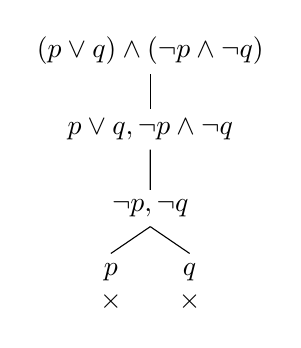
\begin{tikzpicture}[
        level distance=1cm,
        sibling distance=1.5cm,
        level 2/.style={sibling distance=1cm},
        edge from parent path={(\tikzparentnode.south) -- (\tikzchildnode.north)}
      ]
      \node {$(p \lor q) \land (\neg p \land \neg q)$}
        child { 
          node {$p \lor q, \neg p \land \neg q$}
          child { 
            node {$\neg p, \neg q$} 
            child { node[align=center] {$p$ \\ $\times$} }
            child { node[align=center] {$q$ \\ $\times$} }
          }
        };
      \end{tikzpicture}
      }  
    \end{latin}
    \end{center}
  با این حال، ما \emph{جدول معنایی کلاسیک} را ترجیح می‌دهیم زیرا در آن به‌وضوح دیده می‌شود که کدام فرمول‌ها نامزد تجزیه هستند و چگونه برگ‌ها علامت‌گذاری می‌گردند.
  
  \end{example}